	\begin{figure}[H]
		\centering
 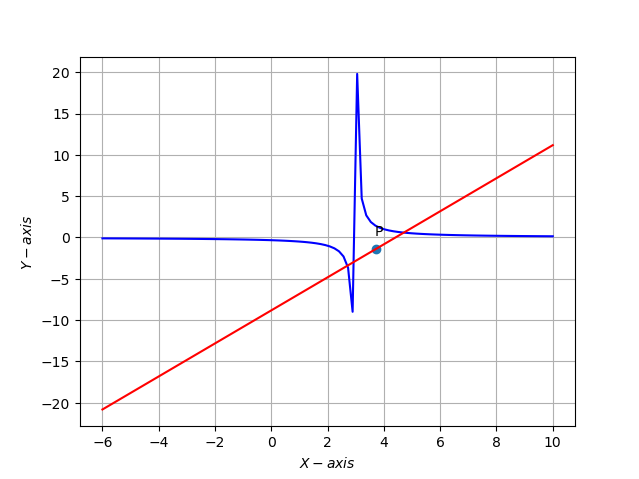
\includegraphics[width=0.75\columnwidth]{chapters/12/6/3/11/figs/con_fig.png}
		\caption{}
		\label{fig:12/6/3/11}
  	\end{figure}
From the given information
\begin{align}
	\vec{V}
	&=\myvec{
		0 &\frac{1}{2}\\\frac{1}{2} & 0\\
	},
\vec{u} = \myvec{
0 \\-\frac{3}{2}
},  f = -1, m=2
	\label{12/6/3/11/eq1}
	\\
	\implies
	\vec{n}&=\myvec{
-m \\ 1 
} = \myvec{-2 \\ 1}  \\
\label{12/6/3/11/eq2}
\end{align}
Hence, the given curve is a hyperbola.
%\raggedright
Substituting  numerical values, we obtain the condition in 
	\eqref{prop:conic-p-contact-nonparab-cond},
which implies that the line with slope 2 is not a tangent.  This can be verified from  
		\figref{fig:12/6/3/11}.
